% Created 2019-04-23 Tue 11:10
% Intended LaTeX compiler: pdflatex
\documentclass[a4paper, 12pt]{article}
\usepackage[utf8]{inputenc}
\usepackage[T1]{fontenc}
\usepackage{graphicx}
\usepackage{grffile}
\usepackage{longtable}
\usepackage{wrapfig}
\usepackage{rotating}
\usepackage[normalem]{ulem}
\usepackage{amsmath}
\usepackage{textcomp}
\usepackage{amssymb}
\usepackage{capt-of}
\usepackage{hyperref}
\usepackage[left=2.5cm, right=2.5cm, top=2.5cm, bottom=2.5cm, bindingoffset=1.5cm, head=15pt]{geometry}
\usepackage{setspace}
\usepackage{caption}
\onehalfspacing
\usepackage[official]{eurosym}
\usepackage{amsmath}
\usepackage{amssymb}
\usepackage{makecell}
\renewcommand\theadalign{cc}
\renewcommand\theadfont{\bfseries}
\renewcommand\theadgape{\Gape[2pt]}
\usepackage{xcolor}
\newcommand{\red}[1]{\textcolor{red}{[#1]}}
\usepackage{lmodern}
\usepackage{xcolor}
\usepackage[newfloat]{minted}
\usepackage{tcolorbox}
\tcbuselibrary{minted}
\usepackage{notation/rl}
\usepackage{notation/model}
\usepackage{template/list}
\let\itemize\hitemize
\usepackage{fancyhdr}
\pagestyle{fancy}
\fancyhead{}
\fancyfoot{}
\fancyhead[LE,RO]{\textsl{\leftmark}}
\fancyhead[RE,LO]{Tobias Richter}
\fancyfoot[C]{\thepage}
\renewcommand{\headrulewidth}{0.4pt}
\renewcommand{\footrulewidth}{0pt}
\usepackage{apacite}
\let\cite\shortcite
\let\textcite\shortciteA
\usepackage[nohyperlinks]{acronym}
\usepackage[bottom]{footmisc}
\interfootnotelinepenalty=10000
\usepackage[notlof,notlot,nottoc]{tocbibind}
\newcommand{\studentID}{558305}
\newcommand{\thesistype}{Master Thesis}
\newcommand{\supervisor}{Univ.-Prof. Dr. Wolfgang Ketter}
\newcommand{\cosupervisor}{Karsten Schroer}
\pagenumbering{Roman}
\author{Tobias Richter}
\date{\today}
\title{Reinforcement Learning Portfolio Optimization of Electric Vehicle Virtual Power Plants}
\hypersetup{
 pdfauthor={Tobias Richter},
 pdftitle={Reinforcement Learning Portfolio Optimization of Electric Vehicle Virtual Power Plants},
 pdfkeywords={},
 pdfsubject={},
 pdfcreator={Emacs 26.1 (Org mode 9.2.1)},
 pdflang={English}}
\begin{document}

\makeatletter
\begin{titlepage}
    \begin{center}
        \vspace*{1cm}

        \Large
        \textbf{\@title{}}

        \vspace{1.5cm}

        \thesistype{}

        \vspace{1cm}

        \begin{figure}[htbp]
             \centering
             
\includegraphics[width=.5\linewidth]{./fig/UoC-logo.png}
        \end{figure}

        \vspace{1cm}

        \large
        \textbf{Author}: \@author{} (Student ID: \studentID{})\\
        \large
        \textbf{Supervisor}: \supervisor{}\\
        \large
        \textbf{Co-Supervisor}: \cosupervisor{}

        \vspace{1cm}
        \large
        Department of Information Systems for Sustainable Society\\
        Faculty of Management, Economics and Social Sciences\\
        University of Cologne\\

        \vspace{1cm}
        \@date{}

    \end{center}
\end{titlepage}
\makeatother
\clearpage
\thispagestyle{empty}
\section*{Eidesstattliche Versicherung}
\label{sec:SOOA}

\vspace{2.5cm}

% Statement of original authorship - Needs to be in German
% see also here: https://www.wiso.uni-koeln.de/sites/fakultaet/dokumente/PA/formulare/eidesstattliche_erklaerung.pdf

Hiermit versichere ich an Eides statt, dass ich die vorliegende Arbeit selbstständig und ohne die Benutzung anderer als der angegebenen Hilfsmittel angefertigt habe. Alle Stellen, die wörtlich oder sinngemäß aus veröffentlichten und nicht veröffentlichten Schriften entnommen wurden, sind als solche kenntlich gemacht. Die Arbeit ist in gleicher oder ähnlicher Form oder auszugsweise im Rahmen einer anderen Prüfung noch nicht vorgelegt worden. Ich versichere, dass die eingereichte elektronische Fassung der eingereichten Druckfassung vollständig entspricht.

\vspace{1cm}

\noindent
Die Strafbarkeit einer falschen eidesstattlichen Versicherung ist mir bekannt, namentlich die Strafandrohung gemäß § 156 StGB bis zu drei Jahren Freiheitsstrafe oder Geldstrafe bei vorsätzlicher Begehung der Tat bzw. gemäß § 161 Abs. 1 StGB bis zu einem Jahr Freiheitsstrafe oder Geldstrafe bei fahrlässiger Begehung.

\vspace{3cm}
\noindent
\textbf{Tobias Richter}

\vspace{0.5cm}
\noindent
Köln, den 01.05.2019
\clearpage
\thispagestyle{empty}

\section*{Abstract}
This is an abstract

\begin{itemize}
\item One or two sentences providing a basic introduction to the field, comprehensible to a scientist in any discipline.
\item Two to three sentences of more detailed background, comprehensible to
scientists in related disciplines.
\item One sentence clearly stating the general problem being addressed by this particular study.
\item One sentence summarising the main result (with the words “here we show” or their equivalent).
\item Two or three sentences explaining what the main result reveals in direct comparison to what was thought to be the case previously, or how the main result adds to previous knowledge.
\item One or two sentences to put the results into a more general context.
\item Two or three sentences to provide a broader perspective, readily comprehensible to a scientist in any discipline, may be included in the first paragraph
\end{itemize}

\begin{center}
\includegraphics[width=.9\linewidth]{./fig/abstract.png}
\end{center}
\clearpage

\setcounter{page}{1}
\tableofcontents
\clearpage
\listoffigures
\clearpage
\listoftables
\clearpage

\section*{List of Abbreviations} \markboth{LIST OF ABBREVIATIONS}{}
\begin{acronym}[GCRM]
	\acro{ANN}{Artificial Neural Network}
	\acro{DP}{Dynamic Programming}
	\acro{DSO}{Distribution System Operator}
	\acro{DDQN}{Double Deep Q-Networks}
	\acro{EPEX}{European Power Exchange}
	\acro{EV}{Electric Vehicle}
	\acro{GCRM}{German Control Reserve Market}
	\acro{MC}{Monte Carlo}
	\acro{ML}{Machine Learning}
	\acro{MDP}{Markov Decision Process}
	\acro{PDF}{Probability Density Function}
	\acro{RES}{Renewable Energy Sources}
	\acro{RL}{Reinforcement Learning}
	\acro{TD}{Temporal-Difference}
	\acro{TSO}{Transmission System Operator}
	\acro{V2G}{Vehicle-to-Grid}
	\acro{VPP}{Virtual Power Plant}
\end{acronym}
\clearpage
\section*{Summary of Notation} \markboth{SUMMARY OF NOTATION}{}
Capital letters are used for random variables, whereas lower case letters are used for
the values of random variables and for scalar functions. Quantities that are required to
be real-valued vectors are written in bold and in lower case (even if random variables).
\begin{tabbing}
    \=~~~~~~~~~~~~~~~~~~  \= \kill
    \>$\defeq$            \> equality relationship that is true by definition\\
    \>$\approx$           \> approximately equal\\
    \>$\E{X}$             \> expectation of a random variable $X$, i.e., $\E{X}\defeq\sum_x p(x)x$\\
    \>$\Re$               \> set of real numbers\\
    \>$\leftarrow$        \> assignment\\
    \\
    \>$\e$                \> probability of taking a random action in an \e-greedy policy\\
    \>$\alpha$            \> step-size parameter\\
    \>$\gamma$            \> discount-rate parameter\\
    \>$\lambda$           \> decay-rate parameter for eligibility traces\\
    \\
    \>$s, s'$             \> states\\
    \>$a$                 \> an action\\
    \>$r$                 \> a reward\\
    \>$\S$                \> set of all nonterminal states\\
    \>$\A$                \> set of all available actions\\
    \>$\R$                \> set of all possible rewards, a finite subset of $\Re$\\
    \>$\subset$           \> subset of; e.g., $\R\subset\Re$\\
    \>$\in$               \> is an element of; e.g., $s\in\S$, $r\in\R$\\
    \\
    \>$t$                 \> discrete time step\\
    \>$T, T(t)$           \> final time step of an episode, or of the episode including time step $t$\\
    \>$A_t$               \> action at time $t$\\
    \>$S_t$               \> state at time $t$, typically due, stochastically, to $S_{t-1}$ and $A_{t-1}$\\
    \>$R_t$               \> reward at time $t$, typically due, stochastically, to $S_{t-1}$ and $A_{t-1}$\\
    \>$\pi$               \> policy (decision-making rule)\\
    \>$\pi(s)$            \> action taken in state $s$ under {\it deterministic\/} policy $\pi$\\
    \>$\pi(a|s)$          \> probability of taking action $a$ in state $s$ under {\it stochastic\/} policy $\pi$\\
    \>$G_t$               \> return following time $t$\\
    \\
    \>$\p(s',r|s,a)$      \> probability of transition to state $s'$ with reward $r$, from state $s$ and action $a$\\
    \>$\p(s'|s,a)$        \> probability of transition to state $s'$, from state $s$ taking action $a$\\
    \>$\vpi(s)$           \> value of state $s$ under policy $\pi$ (expected return)\\
    \>$\vstar(s)$         \> value of state $s$ under the optimal policy\\
    \>$\qpi(s,a)$         \> value of taking action $a$ in state $s$ under policy $\pi$\\
    \>$\qstar(s,a)$       \> value of taking action $a$ in state $s$ under the optimal policy\\
    \>$V, V_t$            \> array estimates of state-value function $\vpi$ or $\vstar$\\
    \>$Q, Q_t$            \> array estimates of action-value function $\qpi$ or $\qstar$\\
    \\
    \>$d$                 \> dimensionality---the number of components of $\w$\\
    \>$\w$                \> $d$-vector of weights underlying an approximate value function\\
    \>$\hat v(s,\w)$      \> approximate value of state $s$ given weight vector $\w$\\
    \>$\mu(s)$            \> on-policy distribution over states\\
    \>$\MSVEm$            \> mean square value error\\
\end{tabbing}
\clearpage

\pagenumbering{arabic}
\section{Results}
\label{sec:orgf05805e}
The following chapter will cover the main results of this research. First, the
simulation environment is presented. Second, we examine the economic
sustainability of an integrated bidding strategy. Third, the RL approach that
aims to optimize the VPP portfolio is evaluated. In the last section, we will
perform sensitivity analyses on the limiting algorithmic factor, the prediction
accuracy, and a limiting physical factor, the charging infrastructure.

\subsection{Simulation Environment}
\label{sec:org9cbf043}
As part of this research, we developed an event-based simulation platform called
\emph{FleetSim}. The platform allows researchers to develop and test out different
smart charging and bidding strategies in realistic environment based on
real-world data. In FleetSim, intelligent agents (called controllers) centrally
control the charging of an EV fleet, they are responsible to sufficiently charge
their vehicles to satisfy real mobility demand. At the same time, the agents can
create VPP of EVs, provide balancing services to the grid, and take part in
electricity trading. Trips are simulated on an individual level, for example,
not charging an individual EV at a particular point in time, can cause a whole
series of lost rentals, due to an insufficient amount of battery for the next
arriving customers. The agents are evaluated based on the profits of charging
the fleet cheaper than the industry tariff, the costs of losing rentals and the
imbalance they cause if they can not provide market commitments. Additionally,
FleetSim facilitates easy sensitivity analyses, adaption to future market
designs, and integration of novel data sets through its modular architecture and
expandable design (see Figure \ref{fig-fleetsim}). We consider FleetSim as a
research platform for sustainable and smart mobility similar to PowerTac
\cite{ketter16_multiagent_comp_gaming}. It builds on SimPy\footnote{\url{https://pypi.org/project/simpy/}}, a process-based
discrete-event simulation framework. FleetSim is available open source\footnote{\url{https://github.com/indyfree/fleetsim}} and
can be readily installed as a Python package.

\begin{figure}[hp]
\centering
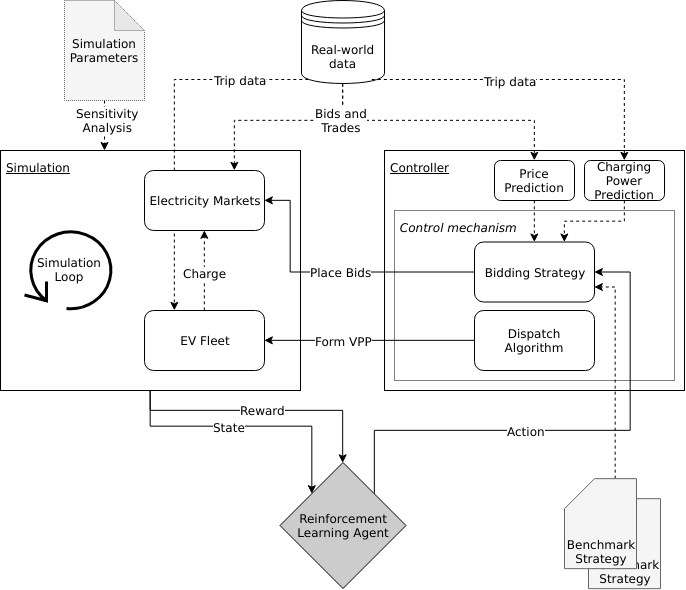
\includegraphics[width=1\linewidth]{fig/simulation-platform.png}
\caption[FleetSim Architecture]{Architecture of FleetSim \label{fig-fleetsim}}
\end{figure}

In order to simplify comparability and focus to real-world applicability of the
analysis, we set the same parameters for all conducted experiments (see Table
\ref{table-sim-params}). They are corresponding to the real Car2Go specifications
described in Chapter \ref{sec-data-car2go}. Further, we fixed the unknown
prediction accuracy of the fleets available charging power \(\fPhat{}\) to an
estimate of modern forecast algorithms performance. The impact of the
predictions uncertainty on the results will later be determined in a sensitivity
analysis.

\begin{table}[hp]
\caption[Simulation Parameters]{Simulation Parameters \label{table-sim-params}}
\centering
\begin{tabular}{lr}
\hline
\hline
Parameter & Value\\
\hline
EV battery capacity (\(\Omega\)) & 17.6 \(\kwh\)\\
EV charging power   (\(\gamma\)) & 3.6 \(\kw\)\\
EV range & 145 km\\
Industry electricity price  (\(p^{ind}\)) & 0.15\footnotemark \(\ekwh\)\\
EV rental tariff & 0.24\footnotemark \(\frac{\eur}{\text{min}}\)\\
EV long distance fee (\(>\text{200 km}\)) & 0.29\textsuperscript{\ref{org35c3348}} \(\frac{\eur}{\text{km}}\)\\
\hline
Prediction accuracy \(\fPhat{}\) week ahead & 70\%\\
Prediction accuracy \(\fPhat{}\) 30 min ahead & 90\%\\
\hline
\hline
\end{tabular}
\end{table}\footnotetext[3]{\label{org92c627e}Average prices of electricity for the industry with an annual consumption
of 500 MWh - 2000 MWh in Germany 2017 \cite{bmwi.19_prices_german}.}\footnotetext[4]{\label{org35c3348}Rental fees according to the Car2Go pricing scheme. See
\url{https://www.car2go.com/media/data/germany/legal-documents/de-de-pricing-information.pdf},
accessed 15\textsuperscript{th} March 2019.}

\subsection{Integrated Bidding Strategy}
\label{sec:org78dd39e}
Research Question 1 examines whether a fleet operator can use a VPP portfolio of
EVs to profitably bid on multiple electricity markets. In Chapter
\ref{sec-model-mechanism}, we proposed a central control mechanism that charges
the fleet with an integrated bidding strategy. The following section evaluates
the results of the control mechanism in the simulation environment.

Table \ref{table-sim-stats} shows the descriptive statistics of the fleet
utilization during a simulation run, with data from June 1, 2016 to January
1, 2018. It can be observed that (a) the volatility of EVs parked at a charging
station is remarkably high (large standard deviation), and (b) the fraction of
EVs that can be utilized for VPP activities is diminishing low (3.55\%). It is
apparent that a high uncertainty and the low share of EVs that can possibly
generate profits are challenging the economic sustainability of our proposed
model. Figure \ref{fig-fleet-utilization} shows that despite a changing rental
behavior throughout the day (e.g., rush hour peaks between 7:00-9:00 and
17:00-19:00), the amount of EVs that can utilized for VPP activities is
comparably stable throughout the day.

\begin{figure}[h]
\centering
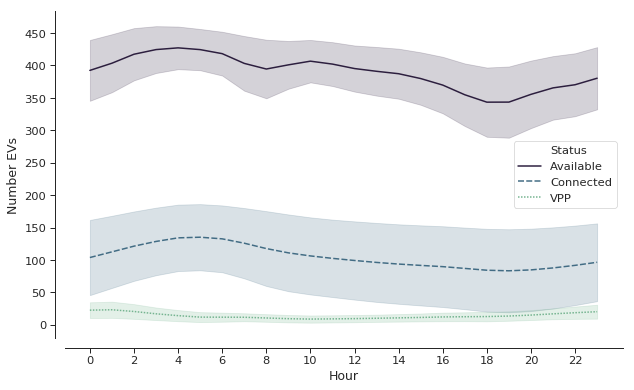
\includegraphics[width=1\linewidth]{fig/fleet-utilization.png}
\caption[Fleet Utilzation]{Daily fleet utilization (average, standard deviation) from June 1, 2016 to January 1, 2018. The blue error band is illustrating the large volatility in the amount of EVs that get parked at a charging station. The share of EVs that can be used as VPP is on average only 3.55\% of the fleet's size. Most of the EVs are either not connected to a charging station or are already fully charged. \label{fig-fleet-utilization}}
\end{figure}

\begin{table}[hp]
\caption[Fleet Statistics]{Fleet Statistics. \label{table-sim-stats}}
\centering
\begin{tabular}{lr}
\hline
\hline
Statistic & Value\\
\hline
Fleet size & 508\\
EVs available (min, max, \textbf{std}) & 389.64 (165, 496, \textbf{49.18})\\
EVs connected (min, max, \textbf{std}) & 61.23 (34, 290, \textbf{61.11})\\
VPP EVs (min, max, \textbf{std}) & 13.84 (0, 94, \textbf{9.01})\\
\hline
\hline
\end{tabular}
\end{table}

We defined several "naive" bidding strategies to evaluate and benchmark the
performance of our developed model. The strategies are naive in that sense that
they are assuming a fixed risk associated with bidding at a specific electricity
market. As opposed to the developed RL agent, they do not take information of
their environment into account and adjust the bidding quantities dynamically.
Instead, the controller discounts the predicted amount of available charging
power with a fixed risk factor \(\lambda\) (see \eqref{eq-model-pb} and
\eqref{eq-model-pi}). Naturally, the controller estimates a higher risk for
bidding on the balancing market week ahead than on the intraday market 30
minutes ahead. We defined following types of strategies:
\begin{enumerate}
\item Risk-averse (\(\lb{}\!=\!0.5\), \(\li{}\!=\!0.3\))

The controller avoids denying rentals and causing imbalances at all costs. In
order to not commit more charging power that it can provide, it places only
bids for conservative amounts of electricity on the markets. The risk-averse
strategies \emph{Balancing} and \emph{Intraday} are comparable to similar strategies
developed by
\textcite{kahlen17_fleet,kahlen18_elect_vehic_virtual_power_plant_dilem}.

\item Risk-seeking (\(\lb{}\!=\!0.2\), \(\li{}\!=\!0.0\))

The controller aims to maximize its profits by trading as much electricity on
the markets as possible. It strives to fully utilize the VPP and allocate a
high percentage of available EVS to charge from the markets. Due to the
rental uncertainty and a low estimated risk, the controller is prone to
offering more charging power to the markets that it can provide. This may
lead to lost rental costs or even imbalances.

\item Full information

The optimal strategy to solve the controlled charging problem. The controller
knows the bidding risks in advance and places the perfect bids on the
markets. In other words, it charges the maximal amount of electricity from
the markets without having to deny rentals or causing imbalances due to
prediction uncertainties.
\end{enumerate}

In Table \ref{table-profits}, the simulation results of all tested strategies are
listed. As expected, the developed integrated bidding strategies outperform
their single market counterparts. The controller is able to capitalize on the
most favorable market conditions and better utilizes the VPP by buying more
electricity from the markets than charging the EVs regularly. The integrated
strategies are resulting in 49\%-54\% more profits for the fleet than the single
market strategies.

A controller bidding according to the \emph{Integrated (risk-averse)} strategy, pays
on average \red{$0.10 \ekwh$  How much?} less for charging the fleet than other
risk-averse strategies. A controller with an \emph{Integrated (risk-seeking)}
strategy, is even more profitable, despite having to account for lost rental
profits. On the other side, the controller caused imbalances (highlighted red)
which lead to high (unknown) market penalties or even exclusion from bidding
activities. For this reason, imbalances need to be avoided, regardless of
potential profits from a higher VPP utilization. We expect that the proposed RL
agent learns a bidding strategy, which avoids imbalances while increasing
profits at the same time. The upper bound of the optimal strategy \emph{Integrated
(full information)}.

\red{Balancing power, stability}

{\captionsetup[table]{aboveskip=0.5cm}
\begin{sidewaystable}[hp]
\caption[Bidding strategy outcomes]{Outcomes of naive bidding strategies over a 1.5 year period. Integrated bidding strategies outperform single market strategies. \label{table-profits}}
\centering
\begin{tabular}{l|cccccc}
 & \thead{Balancing\\(risk-averse)} & \thead{Intraday\\(risk-averse)} & \thead{Integrated\\(risk-averse)} & \thead{Integrated\\(risk-seeking)} & \thead{Integrated\\(full information)}\\
\hline
\hline
VPP utilization (\%) & 39 & 47 & 62 & 81 & 71\\
Energy bought (MWh) & 803 & 985 & 1292 & 1681 & 1473\\
Energy charged regularly (MWh) & 1278 & 1096 & 789 & 400 & 608\\
Lost rental profits (1000 \eur) & 0 & 0 & 0 & 15.47 & 0\\
No. Lost rentals & 0 & 0 & 0 & 1237 & 0\\
Imbalances (MWh) & 0 & 0 & 0 & \textcolor{red}{1.01} & 0\\
Average electricity price (\(\ekwh\)) & - & - & - & - & -\\
Gross profit increase (1000 \eur) & 43.62 & 45.08 & \textbf{67.04} & \textbf{72.51} & 77.36\\
\hline
\hline
\end{tabular}
\end{sidewaystable}

}

\subsection{Reinforcement Learning Portfolio Optimization}
\label{sec:orgbec57b9}
Research Question 2 investigates whether a RL agent can optimize the integrated
bidding strategy by dynamically adjusting the bidding quantities. The bidding
quantities \(\Pb{}, \Pi{}\) are based on the evaluated risk associated with
bidding on the individual electricity markets. In Chapter \ref{sec-model-rl}, we
introduced a RL approach that learns the risk factors \(\lb{}\), \(\li{}\) based on
its observed environment and received reward signals. In Appendix
\ref{app-rl-hyperparams}, the hyperparameters are presented which we used to train
the dueling DDQN algorithm and solving the controlled charging problem under
uncertainty. The values were determined manually through experimentation for the
best results. The speed of convergence was also used as a criterion, since the
training environment Google Colaboratory only allows up to 12 hours of computing
time.

Further, the imbalance costs \(\beta\) were set to an artificially high value to
incentivize the agent to learn to always avoid imbalances. Whenever the agents
takes an action that causes imbalances (i.e., bid too much electricity), it will
receive a highly negative reward signal, leading to a low estimated Q-value of
that chosen action in a specific state.

\begin{figure}[h]
\centering
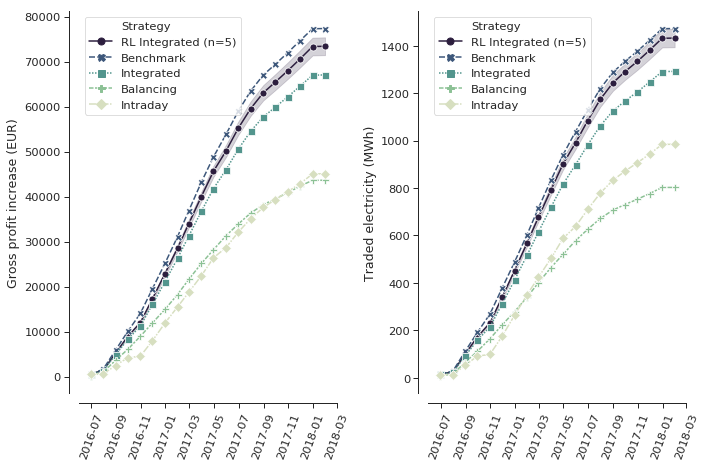
\includegraphics[width=1\linewidth]{fig/rl-results.png}
\caption[Comparison of gross profit results]{Comparison of gross profits and traded electricity between the proposed optimized integrated strategy and the other three naive charging strategies. The RL algorithm improves the achieved gross profit increase of the integrated bidding strategy on average by 12\% and accomplishes nearly optimal results when compared to the benchmark strategy. \label{fig-rl-profits}}
\end{figure}

In Figure \ref{fig-rl-profits}, the performance of the optimized integrated
bidding strategy is presented. The proposed RL algorithm increases the gross
profits of the fleet on average (n=5) by approximately 72-75\% when compared with
the naive single market strategies and by approximately 12\% when compared with
the naive integrated strategy. In none of the tested strategies the controller
procured more electricity from the market that it can charge. To reach the
optimal solution the gross profits would need to be increased by 3\% further.
Similarly, the RL algorithm increases the amount of electricity that the fleet
charges from the electricity markets while avoiding imbalance at the same time.
\red{Balancing power, renewables}

In another experiment, we evaluated the performance of the proposed RL algorithm
in comparison to other RL algorithms with a simpler architecture. In particular,
we were interested what impact modern advances in deep RL have on the ability to
quickly learn to improve the agents policy, while still achieving good results
after the whole training period. This question is especially relevant for the
case, when no prior training for the fleet controller is possible and the agent
has to quickly learn to avoid procuring more energy from the markets that it can
charge. Therefore, we removed the notion of imbalance costs and changed the
simulation setup to instantly stop the training episode when imbalances occur.
In this way, the agents learns to maximize its reward while circumventing
imbalances at all costs. The agent achieves a higher reward the longer it trades
electricity on the markets without committing to charge more electricity than it
can. We compared the DQN algorithm
\cite{mnih15_human_level_contr_throug_deep_reinf_learn} with the Double DQN
algorithm \cite{hasselt16_deep_reinf_learn_doubl_q_learn} with and without the
dueling architecture \cite{wang15_duelin_networ_archit_deep_reinf_learn}. In
Figure \ref{fig-rl-learning}, the average (n=5) learning performances of the
different RL approaches are displayed.

\begin{figure}[h]
\centering
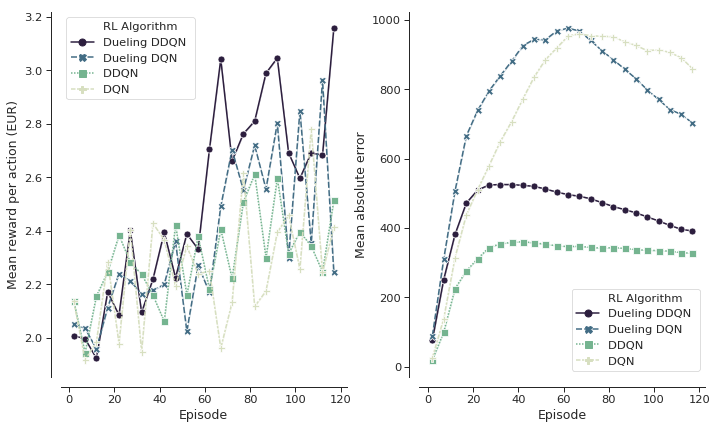
\includegraphics[width=1\linewidth]{fig/rl-learning.png}
\caption[Comparison of RL algorithm learning performance]{Comparison of the learning performance between the proposed RL algorithm and the other three simpler algorithms, averaged over 5 training attempts. Each training period is performed in 1.5 years simulation time with real world data. The dueling DDQN algorithm (dark blue line) learns faster, and achieves better end results than prior algorithms. \label{fig-rl-learning}}
\end{figure}

The experiment shows that the dueling DDQN algorithm learns the fastest and
shows a large increase in mean reward per action after roughly 60 episodes
(about 227 days of simulation time) of training. The dueling DDQN algorithm
shows the largest reward increase and highest reward per action after the whole
training period, which makes it the best algorithm to solve the charging
problem. Despite that it still has a larger mean absolute error than the DDQN
algorithm, indicating that it is more likely to cause imbalances with the
dueling architecture than without. None of the algorithms determined a policy
that never caused imbalances after training on the full 1.5 years of simulation
time (about one hour computing time). In other words, without prior training
with existing data the RL agent would need more than one and a half years to
learn to avoid imbalances. A possible explanation is the problem of learning
from long delayed rewards, first discussed by
\textcite{watkins89_learn_from_delay_rewar}. Long delayed rewards increase the
difficulty of RL problems, since the agent needs to connect occurring decision
outcomes to specific actions way back in the past. In the case of the presented
controlled fleet charging problem, this effect is especially pronounced because
a negative reward signal (caused imbalances) can occur up to 672 timesteps (one
week) after the agent decided on the bidding quantity for the balancing market,
whereas the reward signals from the intraday market occur almost immediately
after 2 timesteps (30 minutes).

In summary, both experiments show that our approach is able to learn a
profit-maximizing bidding strategy under varying circumstances, without using
any a priori information about the EV rental patterns. The proposed control
mechanism improves existing approaches and the RL agent can successfully
optimize the VPP portfolio strategy by estimating the risk that is associated
with bidding on the markets.

\subsection{Sensitivity Analysis}
\label{sec:orge692fde}
The ability to accurately forecast the available fleet charging power plays an
important role in determining the optimal bidding quantity to submit to the
markets. If the fleet controller is certain about the number of connected EVs
that it can use for VPP activities in the future, it can aggressively trade the
available charging power on the markets, without being concerned about turning
away customers or facing the risk of not being able to charge the committed
amount of electricity. In our previous experiments, we assumed a fixed
prediction accuracy that we set to an estimate of what modern mobility demand
forecasts algorithms can achieve. In order to test the robustness of the results
and their dependence on the prediction accuracy, we conducted a sensitivity
analysis. Therefore, we tested the previously introduced RL approach with
increasing levels of predecition accuracy, from 50\% to 100\% accuracate forecasts
7 days and 30 minutes ahead.

\begin{figure}[htbp]
\centering
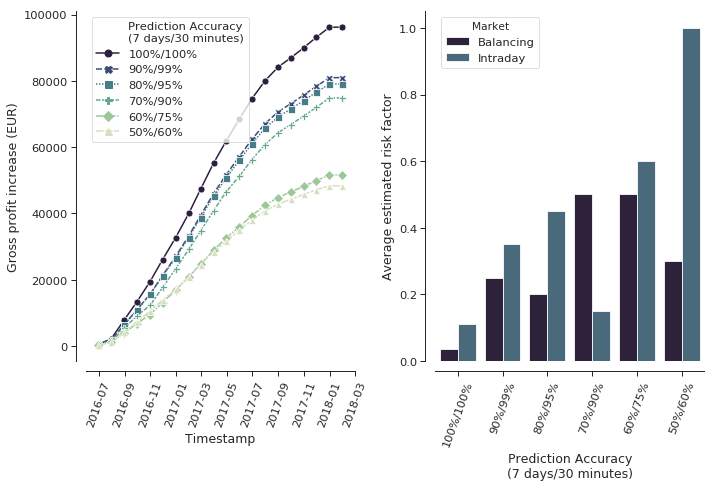
\includegraphics[width=1\linewidth]{fig/rl-accuracy.png}
\caption[Sensivity Analysis: Prediction Accuracy]{Sensivity Analysis: Prediction Accuracy \label{fig-sens-accuracy}}
\end{figure}

In Table \ref{fig-sens-accuracy} the results of the sensitivity analysis are
presented. The left plot shows the effect of the prediction accuracy on the
total gross profit increase, whereas the right plot shows the effect on the
learned risk factors of the RL agent. Intuitively, the realized profit increases
with rising accuracy of the forecasts, while the estimated risk factors decrease
with more accurate forecasts.

Interestingly, the RL agent does not always estimate higher risks for bidding on
the balancing market than on the intraday market,  despite lower accuracy levels
for predicting the available charging power 7 days ahead than 30 minutes ahead.
This result indicates that the RL performance underlies some variations. The
agent succesfully learns to avoid imbalances first by estimating a high total
risk and only later learns to optimize the portfolio by fine-tuning the risk
factors of both markets. We are confident that the agent's limited amount of
training steps is the reason of these variations in learning success and expect
to achieve more robust results with a increased training time.

Also remarkable is the magnitude of the prediction accuracy's effect on the
profit increase. After 1.5 years of simulation time, a RL agent that can rely on
perfect predictions (100\% accuracy) generates almost twice as much profit from
trading electricity than an agent that can only rely on predictions with 50\% and
60\% accuracy, 7 days and 30 minutes ahead respectively. It is striking that the
prediction accuracy has a larger effect (99.13\% profit increase between lowest
and highst accuracy) on the realized profit than the type of bidding strategy
(73.10\% profit increase between worst and best strategy), which we examined in
the previous sections, leaving room for future research.

\clearpage

\section{Conclusion}
\label{sec:org6e58019}
Integrating volatile renewable energy sources into the electricity system
imposes challenges on the electricity grid. In order to ensure grid stability
and avoid blackouts, balancing power is needed to match electricity supply and
demand. Balancing power can be provided by VPPs that generate or consume energy
within a short period of time and offer these services on the electricity
markets \cite{pudjianto07_virtual_power_plant_system_integ}. EV fleet operators
can utilize idle vehicles to form VPPs and offer available EV battery capacity
as balancing power to the markets. The fleet can offer balancing services
directly via tender auctions on the balancing market or via continuous trades on
the intraday market, where participants procure or sell energy to self-balance
their portfolios \cite{pape16_are_fundam_enoug}. Both markets have complementary
properties in terms of price levels and lead times to delivery, which motivates the
creation of a VPP portfolio to profitably participate in both markets and extend
the business model of the fleet.

However, there are certain risks associated  with this business model extension.
EVs can only be allocated to a VPP portfolio if they are connected to a charging
station and have sufficient free battery capacity available, information which
is unknown to the fleet at the time of market commitment. This uncertainty makes
it difficult for fleet operators to estimate the size of the VPP and calculate
the optimal bidding quantities. Moreover, if fleet operators offer more
balancing power than they can provide, they face high imbalance penalties from
the markets. For a sustainable business model fleet operators also need to
balance VPP activities with their primary offering, customer mobility. Denying
customer rentals to ensure that the fleet can fulfill the market commitments,
results in opportunity costs of lost rentals that compromise the profitability
of the fleet.

In the following chapter, we will summarize the conducted research of this
thesis to address the aforementioned challenges. Furthermore, the contribution
of this work is outlined and the main results are presented and discussed.
Finally, we list specific limitations of this study and give insights on further
areas of research.
\subsection{Contribution}
\label{sec:org407ae8b}
The core contributions of this thesis are the following: First, we
conceptualized a DSS for controlled EV charging under uncertainty. The DSS
constitutes the core of a business model extension for fleet operators to manage
a VPP portfolio of EV batteries. A controlled charging problem has been
mathematically formulated and a control mechanism introduced that aims solve the
proposed problem. Second, we developed an event-based simulation platform that
facilitates fleet management research with real-world data. We evaluated various
baseline bidding strategies within the simulation platform and tested out the
behavior of intelligent agents in the context of controlled EV charging. Third,
we proposed a novel integrated bidding strategy that offers balancing services
of a VPP portfolio to multiple electricity markets simultaneously. Instead of
submitting only conservative amounts of battery capacity to a single market,
like previous studies did
\cite{kahlen17_fleet,kahlen18_elect_vehic_virtual_power_plant_dilem}, our proposed
strategy aims to maximize profits by procuring electricity from the multiple
markets to the greatest extent possible without causing imbalances. Forth, we
proposed the usage of a RL agent that learns to optimize the composition of the
VPP portfolio and the associated risks of bidding on the markets. The agent
dynamically determines risk factors, depending available and predicted fleet
information and market conditions. Therefore, we formulated a MDP that is
designed for agents to work in previously unknown environments and uncertain
conditions. The RL approach was developed with the focus on real-world
applicability, fast convergence rates and generalizability. We expect the
proposed approach to work in a variety of different settings, with different
kinds of EVs (e.g., electronic bikes), independent of the geographical location
of the fleet.

The proposed method was evaluated in a series of expriments with real-world
carsharing data from Car2go in Stuttgart and German electricity market data from
June 2017 until January 2018. The results show that the developed method
improves existing approaches and would increase the gross profits of the fleet
by roughly \(78 000\; \eur\) over a 1.5 year period. Since free float carsharing
has inherently uncertain demand patterns, better results are expected with other
kinds of EV fleets. We found that the integrated bidding strategy generates
49\%-54\% more profits, compared to the naive benchmark strategies. Fleet
controllers following the integrated bidding strategy, can mitigate risks and
increase profits by exploiting market properties of both markets. Further, we
showed that the proposed RL agent can optimize the integrated bidding strategy
under uncertainty by roughly 15\%, almost \red{how much?} reaching the optimal
solution with full information available. The agent was able to successfully
estimate the bidding risk, avoid imbalances and keeping lost rentals to a
minimum. \red{Balancing power, stabilized the grid} Additionally, we tested and
compared the performance of modern RL algorithms and found that recent advances
in deep RL do improve the robustness and convergence rates in real-world
applications. Despite these improvements, all RL approaches needed more than 1.5
years of simulation time to learn to avoid imbalances penalties, which makes RL
agents unsuitable to deploy in unseen fleet environments without prior training
data. A sensitivity analysis of the prediction accuracy of the fleet balancing
power showed that the accuracy has large impact on the fleet profitability. If
the controllers predictions are very uncertain, the RL agent estimates high
bidding risks and can only offer conservative amounts of balancing power on the
markets. Surprisingly, the effect of prediction accuracy on the total gross
profit increase is larger than the choice of bidding strategy or RL algorithm
architecture, which leaves room for future research.


\begin{itemize}
\item Integrated bidding strategy exploit multiple markets properties
\item Online learning algorithm (difference? -- real data?)
\item Advantage over forecast like Kahlen: General, unseen, etc..
\end{itemize}


Impact on grid: Balancing power, mention balancing power.

Discuss:
\begin{itemize}
\item Compare to other studies!
\begin{itemize}
\item Fleet Charging
\begin{itemize}
\item No uncertainty
\item Only one market
\item No sensitivity on accuracy prediction (We found very important)
\end{itemize}
\item Other approaches (VPP, stochastic)
\cite{kahlen18_elect_vehic_virtual_power_plant_dilem} (no imbalance costs!)
\cite{vandael15_reinf_learn_heuris_ev_fleet}
\end{itemize}

\item Discuss results?
\begin{itemize}
\item Gross profits small - Mention before?
\item Policy
\item Investment
\item V2G?
\item Market Setup
\end{itemize}
\end{itemize}

\subsection{Limitations}
\label{sec:org2f54612}
\begin{itemize}
\item Model:
\begin{itemize}
\item Bidding Mechanism: one week ahead, always accepted
\item Policy \& Regulation: EVs not allowed to provide balancing power, minimum
bidding quantities 1MW.
\item Markets: Fleet is a price-taker, what about larger fleets? Simulate market influence
\item Deny rentals only in the same market period (More deny, less imbalance)
\end{itemize}
\item RL: See \cite{vazquez-canteli19_reinf_learn_deman_respon} conclusion for
limitations.
\begin{itemize}
\item Training time in real time. Generalization to other cities?
\end{itemize}
\end{itemize}
\subsection{Future Research}
\label{sec:org144ab16}

\begin{itemize}
\item This result shows that leaving promising room for future research of highly
\end{itemize}
accurate mobility demand algorithms.
\begin{itemize}
\item Model:
\begin{itemize}
\item Investigate modern/current market design, that changed their bidding
mechanisms to to better integrate renewable energy generators.
\begin{itemize}
\item Daily/Day-ahead tenders with 4 hour market periods.
\end{itemize}

Mischpreisverfahren

i.e. daily w/ 4h slots. German "Mischpreisverfahren"
\end{itemize}
\item RL: Long-delayed rewards, different reward structure, memory based
\item Prediction Algorithms improvement, reference to sensitivity analysis
\end{itemize}

\clearpage
\end{document}
